V tomto projektu vidím potenciál jak z osobního, tak i profesního hlediska.

Z osobního pohledu mě motivuje příležitost k sebevzdělávání, protože mě zajímá kompletní vedení projektu od počáteční myšlenky až k jeho realizaci.
Rád bych se aktivně zapojil do všech fází – od návrhu přes vývoj po řešení různých problémů.

Z profesního hlediska mě přitahuje vývoj těchto technologií, protože věřím, že v budoucnu budou mít klíčový význam.
To by mohlo zvýšit atraktivitu tohoto projektu, a časem by mohl přitáhnout pozornost investorů.
Například by jej mohl chtít financovat některý zemědělec, pod  podmínkou vývoje, implementace a podpory na jeho farmě, což by mi přineslo mnoho cenných zkušeností.

Na základě těchto úvah plánuji v projektu pokračovat a dále jej rozvíjet.
Níže uvádím funkcionality, které mám v úmyslu implementovat po dokončení této práce.\newline

\section{Koncept identifikace nejlepší nosnice}\label{sec:koncept-identifikace-nejlepsi-nosnice}

Při chovu slepic by bylo velmi užitečné vědět, kolik vajec která slepice snáší, protože to umožňuje farmáři sledovat produktivitu jednotlivých slepic.
Díky tomu může:
\begin{itemize}
    \item Optimalizovat chov: Identifikací slepic s vysokou a nízkou snáškou může farmář rozhodnout o selekci nebo o zvláštní péči pro méně produktivní slepice.
    \item Zlepšit zdraví slepic: Nízká snáška může být indikátorem zdravotních problémů. Včasná identifikace umožňuje podniknout kroky k léčbě nebo prevenci nemocí.
    \item Efektivněji plánovat krmení a zdroje: Sledování výkonu pomáhá v rozhodování o výživě a péči, aby byla maximalizována produkce vajec při optimálních nákladech.
    \item Zvýšit ziskovost: Monitorováním snášky lze zlepšit celkovou produktivitu farmy a tím i její ekonomickou efektivitu.
\end{itemize}

Celkově tedy znalost počtu vajec od každé slepice pomáhá v efektivním řízení chovu a zajišťuje lepší výsledky jak po stránce produkční, tak ekonomické.
Abych toho dosáhl, potřebuji být schopen jednotlivé slepice identifikovat a tuto informaci propojit s momentum, kdy slepice sense v kurniku vejce.
V sekci  pridat odkaz  “Vaha”, je popsan mechanismus, kdy pravidelnou analyzou casove rady, kterou poskytuje vaha ziskame informaci o casove udaji, kdy bylo vejce sneseno.
Pak jiz jen staci identifikovat, ktera z nasich slepic byla v tu dobu v hnízdě.
Existuje několik variant, jak slepice identifikovat, já jsem se rozhodl využít k identifikaci obrazovou analýzu.
Postupuji následujícím způsobem.
Nejprve procházím videozáznam a identifikuji oblasti, kde se slepice nacházejí.
Tyto oblasti následně vystřihnu a uložím do samostatných souborů.
Poté procházím tyto menší obrázky a pomocí segmentace vystřihnu plochu, kde je slepice, zatímco ostatní části zůstanou bílé.
Takto vyříznuté obrázky převádím na tenzory.
Převod na tenzor znamená, že dvourozměrný obraz (matice pixelů) převedu do vícerozměrné datové struktury, která dokáže reprezentovat různé vlastnosti obrazu a je vhodná pro strojové učení a další matematické zpracování.
Tímto způsobem získám numerickou reprezentaci obrazu, se kterou mohu efektivně pracovat.
Získané tenzory porovnávám se vzorovými vektory uloženými v databázi.
Pokud je vektor shodný, znamená to, že jsem našel odpovídající slepici, a podařilo se mi ji tak identifikovat.

Algoritmus tedy na počátku vezme jako vstup obrázek z kamery viz obrázek~\ref{fig:source_chick_image}.
Dále je obrázek segmentován a jsou vyjmuty pouze tvary, které algoritmus vyhodnotil jako slepice viz obrázek~\ref{fig:segmented_chicks2}.
Na závěr je pro každý výřez vypočítán tenzor na jehož základě jsou slepice roztřízeny do jednotlivých skupin podle barvy viz obrázek~\ref{fig:chicks_in_clusters}.



\begin{figure}[h]
    \centering
    \begin{subfigure}[t]{1\textwidth}
        \centering
        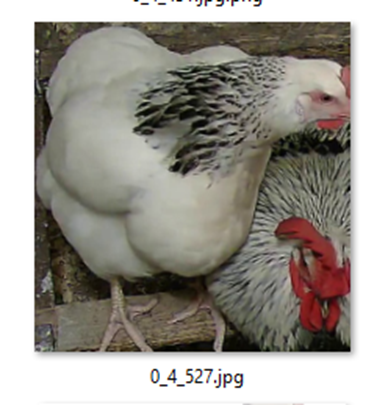
\includegraphics[width=\textwidth]{img/source_chick_image}
        \caption{Jeden ze vstupů do algoritmu pro nosnice}
        \label{fig:source_chick_image}
    \end{subfigure}

    \begin{subfigure}[t]{1\textwidth}
        \centering
        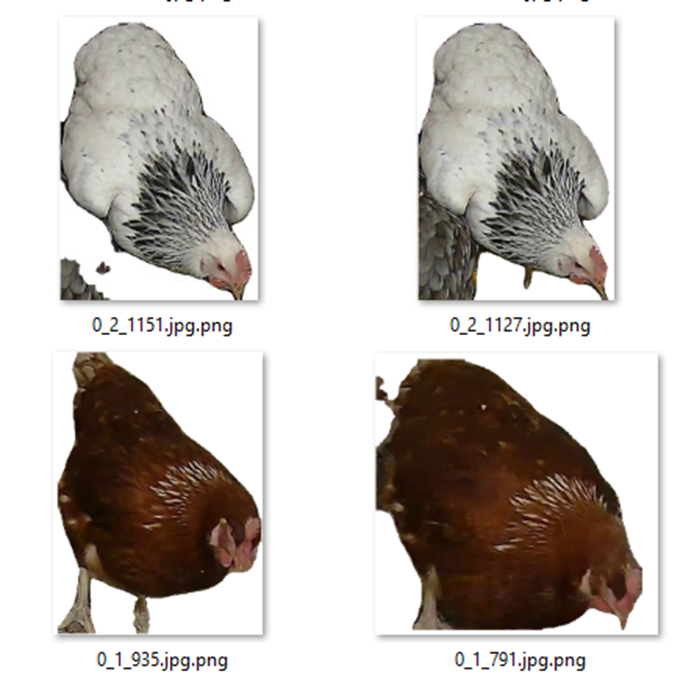
\includegraphics[width=\textwidth]{img/segmented_chicks}
        \caption{Segmentované slepice z fotek}
        \label{fig:segmented_chicks2}
    \end{subfigure}

    \begin{subfigure}[t]{1\textwidth}
        \centering
        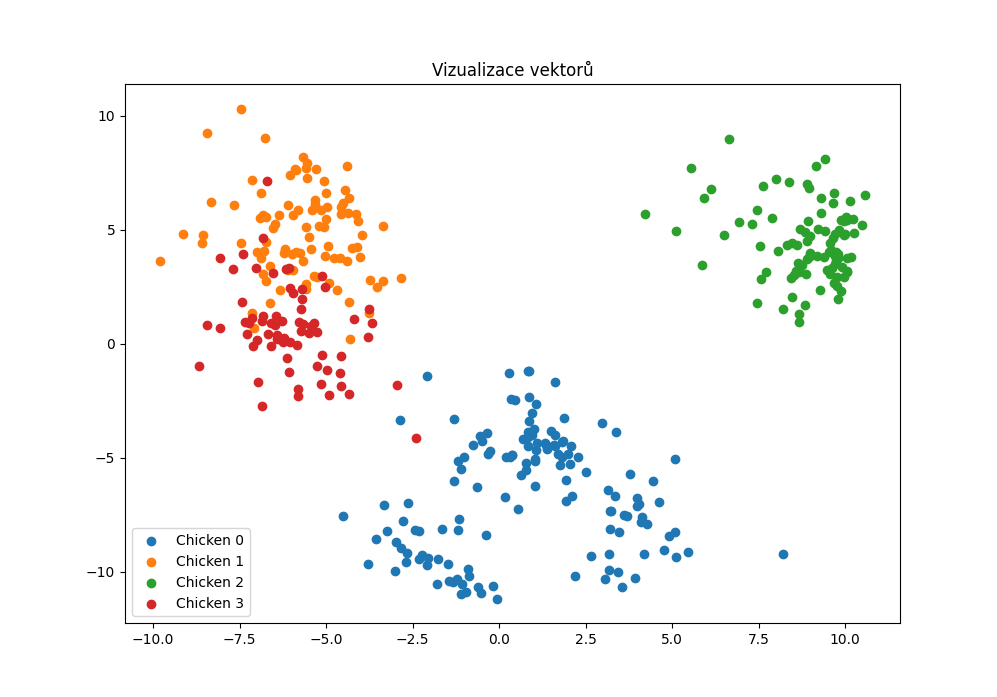
\includegraphics[width=\textwidth]{img/chicks_in_clusters}
        \caption{Algoritmem rozdělené slepice dle tenzorů}
        \label{fig:chicks_in_clusters}
    \end{subfigure}
\end{figure}

\section{Vylepšení konstrukce dvířek}\label{sec:vylepseni-konstrukce-dvirek}
Vylepšení konstrukce dvířek a realizace finálního řešení je jeden z plánů do budoucna pro tento projekt.
Jak již bylo zmíněno v popisu současné konstrukce v sekci~\ref{sec:konstrukce-dvirek}, aktuální konstrukce je příliš drahá na výrobu a také zbytečně robustní.
Pro finální instalaci v následujících větách popíšu návrh na realizaci produkční konstrukce.\newline
Konstrukce by měla být levnější na výrobu i na materiál a zároveň stejně bezpečná a výkonná jako ta stávající prototypová.
Nový rám bude tvořen z železných U profilů použitých zároveň jako vodící lišty pro posuv dvířek.
Posuvný plát bude z plastové desky.

\subsection*{Navíjecí mechanismus}\label{subsec:navijeci-mechanismus}
Způsob ovládání neboli napájení se nemění takže není třeba dělat žádné úpravy na řídící jednotce popsané detailněji v sekci~\ref{sec:ridici-jednotka}.
Pohyb bude dvířkům dodávat malý elektrický naviják vlastní konstrukce.
Díky vlastnímu návrhu bude možno celý rám navijáku navrhnout pomocí CAD programu a následně ho celý vyrobit na 3D tiskárně.
Tento způsob výroby šetří čas a je zajiště přiměřeně stejná kvalita u všech součástek.
Pohonnou jednotkou navijáku bude 12 V elektromotor model JGA25-370 na stejnosměrné napětí s vestavěnou převodovkou.
Díky převodovce dokáže motor vyvinout kroutící moment až 130N na 1cm dlouhé páce, což je na pohyb dvířek dostačující.
Vývodový hřídel z převodovky elektromotoru bude připevněn k navíjecímu bubnu o průměru okolo 15 mm.
Na navíjecím bubnu bude připevněno i lanko, které se bude používat na vytahování dvířek nahoru.
Pohyb dolů je zajištěn díky gravitaci, díky čemuž stačí povolit lanko a dvířka sama sjedou dolů.
Jako pokračování v ose otáčení motoru a bubnu bude k bubnu připevněn malý šnekový hřídel s maticí.
Matici je zamezeno otáčení opřením o rám navijáku takže se při otáčení hřídele se bude matice posouvat.
Tohoto pohybu bude využívat poslední součást navijáku a to systém dorazů, aby bylo možno nastavit maximální počet otáček bubnu a nedošlo tak k úplnému odvinutí lanka.
Úplné odvinutí lanka by v případě, že by se motor pořád točil, znamenalo, že se lanko zase začne navíjet opačným směrem, což obrátí navíjecí logiku navijáku.
Řídící jednotka totiž počítá pouze s jedním směrem otáčení a nepočítá s náhlým přehozením směru otáček motoru pro navíjení a odvíjení.


%konstrukce dveří - instalováno
%- zdroj 12V
%- rám z
%- naviják je s dvířky přopojen lankem
%- navíjecí systém / systém navijáku
%- 12V motor s převodovkou, rychlostí otáčení 60rpm
%- navíjecí buben vytištěný na 3d tiskárně
%- dorazový systém
%\section{Vylepšení funkcionality služby Room Assistant}\label{sec:vylepseni-funkcionality-sluzby-room-assistant}

// TODO

- lze doimplementovat automatické ovládání světel a dvířek pro případ nefunkčnosti home assistanta
- resi rano otevirani dveri kurniku a vecer zavirani
- Integrace se sluzbou  - https://api.sunrise-sunset.org/json?lat=50\&lng=14.5
- dvere se nezavrou pokud nejsou slepice doma (kontrolu lze provézd zavoláním přímo na chicken watch guarda)
- dvere v modu automatickeho zavirani si volaji o data kdy zavirat https://kodim.cz/czechitas/daweb/js2/server-komunikace/cv-volani-api/vychod-zapad